\section{Aritmetika Modular}

\subsection{Definisi Kongruensi}

Dua bilangan bulat $a$ dan $b$ dikatakan \textbf{kongruen modulo $n$} jika $n$ membagi $(a - b)$. Ditulis:
\[
a \equiv b \pmod{n} \quad \Leftrightarrow \quad n \mid (a - b)
\]

\begin{contoh}
$17 \equiv 2 \pmod{5}$ karena $17 - 2 = 15$ habis dibagi 5. Dengan kata lain, $17 \bmod 5 = 2$.
\end{contoh}

Aritmetika modular membentuk fondasi matematis untuk banyak algoritma kriptografi modern, terutama RSA yang secara fundamental bergantung pada sifat-sifat operasi modulo. Menurut blog 3010tangents, aritmetika modular memungkinkan pasangan tak terhingga dari bilangan untuk memenuhi kendala tertentu, tetapi tidak memungkinkan pengguna untuk mendekripsi pesan tanpa kunci yang tepat. Sifat ini membuat aritmetika modular sangat ideal untuk kriptografi karena menciptakan masalah satu arah (one-way problem) yang mudah dihitung dalam satu arah tetapi sangat sulit dibalik tanpa informasi tambahan.

Analogi jam sering digunakan untuk menjelaskan konsep modular arithmetic di mana jam analog dengan 12 jam secara alami menggunakan operasi modulo 12. Jika jam menunjukkan pukul 11 dan kita ingin mengetahui waktu setelah 4 jam, hasilnya adalah pukul 3, bukan pukul 15, karena dalam sistem 12-jam kita "melilit kembali" setelah mencapai 12. Konsep melilit kembali (wrap-around) ini adalah esensi dari aritmetika modular dan sangat penting dalam kriptografi di mana kita ingin membatasi hasil operasi dalam rentang tertentu.

\subsection{Representasi \texorpdfstring{$\mathbb{Z}_n$}{Z\_n} dan Bilangan Negatif}

Hasil operasi modulo $n$ direpresentasikan sebagai kelas sisa dalam himpunan $\mathbb{Z}_n$ \cite{shoup2009,stanford_numbertheory}. Secara eksplisit, $\mathbb{Z}_n = \{0, 1, \ldots, n-1\}$. Dalam implementasi, nilai negatif sering dinormalisasi dengan:
\[
a \bmod n = ((a \bmod n) + n) \bmod n
\]
sehingga hasil selalu berada di rentang $0$ sampai $n-1$.

\begin{contoh}
$-3 \bmod 11 = 8$ karena $-3 \equiv 8 \pmod{11}$.
\end{contoh}

\begin{figure}[htbp]
  \centering
  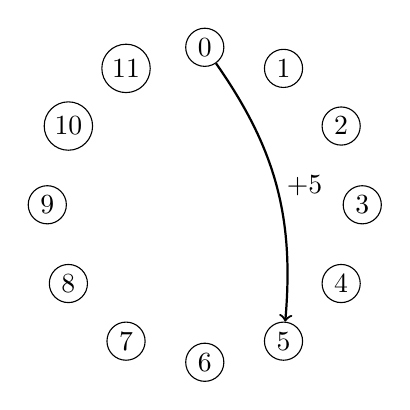
\begin{tikzpicture}[scale=1]
    \foreach \i in {0,...,11} {
      \node[circle, draw, inner sep=2pt] (n\i) at ({90-30*\i}:2) {\i};
    }
    \draw[->, thick] (n0) to[bend left=20] node[midway, right] {$+5$} (n5);
  \end{tikzpicture}
  \caption{Representasi jam aritmetika modular (mod 12).}
\end{figure}

Dalam implementasi kriptografi, representasi $\mathbb{Z}_n$ sangat penting untuk memastikan konsistensi hasil operasi dan mencegah error yang disebabkan oleh nilai negatif atau overflow. Normalisasi nilai negatif dengan menambahkan modulus sebelum mengambil modulo lagi memastikan bahwa semua hasil berada dalam rentang yang diharapkan. Pendekatan ini sangat penting dalam implementasi algoritma RSA di mana operasi modular dilakukan berulang kali pada bilangan yang sangat besar.

\subsection{Operasi Dasar}

Aritmetika modular memenuhi sifat-sifat \cite{trappe2006}:
\begin{itemize}
  \item $(a + b) \bmod n = ((a \bmod n) + (b \bmod n)) \bmod n$
  \item $(a - b) \bmod n = ((a \bmod n) - (b \bmod n) + n) \bmod n$
  \item $(a \cdot b) \bmod n = ((a \bmod n) \cdot (b \bmod n)) \bmod n$
\end{itemize}

\begin{contoh}
$(8 - 13) \bmod 11 = (-5) \bmod 11 = 6$.
\end{contoh}

Sifat distributif aritmetika modular memungkinkan optimasi komputasi yang signifikan dalam implementasi kriptografi, terutama saat bekerja dengan bilangan yang sangat besar seperti dalam RSA. Dengan mengurangi setiap operan terlebih dahulu sebelum melakukan operasi aritmetika, kita dapat mencegah overflow dan meningkatkan efisiensi perhitungan. Teknik ini sangat penting dalam implementasi praktis di mana kita harus melakukan operasi modular berulang kali tanpa kehilangan presisi atau performa.

\subsection{Invers Modular}

Jika $a \cdot x \equiv 1 \pmod{n}$, maka $x$ adalah \textbf{invers modular} dari $a$ modulo $n$, ditulis $x = a^{-1} \pmod{n}$.

\begin{konsep}
Invers modular dari $a$ modulo $n$ hanya ada jika $\gcd(a, n) = 1$. Jika $\gcd(a, n) \neq 1$, maka $a$ tidak memiliki invers modulo $n$.
\end{konsep}

\begin{contoh}
$3^{-1} \equiv 7 \pmod{10}$ karena $3 \cdot 7 = 21 \equiv 1 \pmod{10}$.
\end{contoh}

\begin{table}[htbp]
  \centering
  \small
  \begin{tabular}{cc}
    \toprule
    $a$ & $a^{-1} \bmod 11$ \\
    \midrule
    1 & 1 \\
    2 & 6 \\
    3 & 4 \\
    4 & 3 \\
    5 & 9 \\
    6 & 2 \\
    7 & 8 \\
    8 & 7 \\
    9 & 5 \\
    10 & 10 \\
    \bottomrule
  \end{tabular}
  \caption{Invers modular untuk modulus 11.}
\end{table}

Invers modular merupakan konsep fundamental dalam kriptografi kunci publik, terutama dalam algoritma RSA di mana kunci privat dan publik harus saling invers modulo $\phi(n)$. Menurut Sookocheff, Extended Euclidean Algorithm menyediakan metode efisien untuk menghitung invers modular tanpa harus melakukan pencarian brute force yang tidak praktis untuk bilangan besar. Kemampuan menghitung invers modular dengan cepat dan akurat sangat penting untuk generasi kunci RSA yang aman dan efisien.

\subsection{Pembagian Modular}

Pembagian modular didefinisikan melalui invers: 
\[
\frac{a}{b} \bmod n \equiv a \cdot b^{-1} \bmod n
\]
dengan syarat $\gcd(b, n) = 1$ \cite{rosulek2021}. Jika syarat tidak terpenuhi, pembagian modular tidak terdefinisi.

\begin{contoh}
$4 / 3 \bmod 11 = 4 \cdot 4 \bmod 11 = 5$, karena $3^{-1} \equiv 4 \pmod{11}$.
Sebaliknya, $2 / 6 \bmod 10$ tidak terdefinisi karena $\gcd(6, 10) = 2$.
\end{contoh}

Pembagian modular sangat penting dalam protokol kriptografi modern seperti Diffie-Hellman key exchange dan skema tanda tangan digital. Dalam implementasi praktis, pembagian modular harus dilakukan dengan hati-hati untuk memastikan bahwa pembagi memiliki invers modular sebelum melakukan operasi. Kegagalan memeriksa syarat $\gcd(b, n) = 1$ dapat menyebabkan error runtime atau hasil yang tidak diharapkan dalam aplikasi kriptografi.
